\documentclass[12pt]{article}
\usepackage[utf8]{inputenc}
\usepackage{amsmath}
\usepackage{amssymb}
\usepackage{amsthm}
\usepackage{tikz-cd}
\usepackage{tikz}
\usetikzlibrary{trees}

\newtheorem{theorem}{Theorem}
\newtheorem{lemma}[theorem]{Lemma}
\newtheorem{corollary}[theorem]{Corollary}
\newtheorem*{exercise}{Exercise}
\newtheorem*{definition}{Definition}
\newtheorem*{remark}{Remark}

\newcommand{\legendre}[2]{\genfrac{(}{)}{}{}{#1}{#2}}

\title{Week 12 Lecture Notes: Binary Quadratic Forms}
\author{Edward Zeng}
\date{April 16, 2019}

\begin{document}
\maketitle

\section{Notation}
Unless specified by context or otherwise:
\begin{itemize}
    \item variables are integers
    \item $p$ and $q$ are \textbf{primes}
\end{itemize}

\section{Overview}
Call a function a \textbf{binary quadratic form} (or simply, a \textbf{form}) if
\begin{equation}
    f(x,y) = ax^{2} + bxy + cy^{2}
\end{equation}
We say $f$ \textbf{represents} $n$ if $f(x,y) = n$ for some $x$, $y$. Here, we will be mainly concerned with what numbers a given form can represent, or the \textbf{representations} of a form. Two important results:
\begin{itemize}
    \item There is a connection between the representations of a form and quadratic residues, allowing us to treat a more familiar problem.
    \item We can reduce forms but keep its representation invariant.
\end{itemize}

\section{Preliminaries}
\subsection{Definite and Indefinite Forms}
It is natural to classify forms $f$ by whether it can represent positive numbers, negative numbers, or both:
\begin{itemize}
    \item If $f(x,y) \geq 0$, we call this \textbf{positive semi-definite}.
    \item If $f(x,y) \leq 0$, we call this \textbf{negative semi-definite}
    \item $f$ is \textbf{indefinite} if it can represent both positive and negative integers.
\end{itemize}
A semi-definite form becomes \textbf{definite} if it is equal to zero only when $x = y = 0$.

\subsubsection{}
Let us return to equation (1). It is not hard to see the following implications:
\begin{itemize}
    \item If $f$ is definite, then $a$ and $c$ are nonzero and have the same sign.
    \item If $f$ is semi-definite, then $a$ and $c$ have the same sign (can be zero).
    \item If $f$ is indefinite, no such inferences can be made (although later we will see we can say something if more information is given).
\end{itemize}

\subsection{More Notation}
For the rest of these notes, $a$, $b$, and $c$ used without explanation will denote the coefficients of binary forms.

\subsection{Discriminant}
It is natural to complete the square to determine if a form can take positive or negative values. If we do so in the usual way and assume $a$ is \textit{nonzero}, we have:
\begin{equation}
    f(x,y) = a(x + \frac{b}{2a}y)^{2} - (b^{2}-4ac)(\frac{y}{2a})^{2}.
\end{equation}
Recall $b^{2}-4ac$ is the \textbf{discriminant} of the quadratic equation $ax^{2} + bx + c$. We extend this definition to binary quadratic forms (both zero and nonzero $a$), and denote the discriminant as $d$. An analysis of (2) shows that if $a$ is nonzero, then:
\begin{itemize}
    \item $f$ is definite $\iff$ $d < 0$
    \item $f$ is indefinite $\iff$ $d > 0$
    \item $f$ is semi-definite $\iff$ $d = 0$
\end{itemize}
It is not hard to check that the above statement holds for $a = 0$, and hence does not depend on any extra assumptions.
\begin{remark}
    As negating a negative definite gives a positive definite, we will ignore negative definite forms. Hence from now on, a definite form is synonymous with a positive definite form.
\end{remark}

\subsection{Review}
Before we proceed deeper into theory, we call attention to a useful and intuitive property of quadratic residues that can be a little tricky to prove.
\begin{lemma}
    If $(m, n) = 1$, then the following are equivalent:
    \begin{itemize}
        \item $r$ is a quadratic residue mod $mn$
        \item $r$ is a quadratic residue mod $m$ and mod $n$
    \end{itemize}
\end{lemma}
\begin{proof}
The first statement clearly implies the second. Suppose the second statement is true. Then there exists $a$, $b$ such that
\begin{equation*}
    r \equiv a^{2} \pmod{m}, \quad r \equiv b^{2} \pmod{n}.
\end{equation*}
By the Chinese Remainder theorem, $a$ (mod $m$) and $b$ (mod $n$) lift to a unique $c$ (mod $mn$). Note
\begin{equation*}
    c^{2} \equiv r \pmod{m}, \quad c^{2} \equiv r \pmod{n}
\end{equation*}
hence again by the Chinese Remainder Theorem
\begin{equation*}
    c^{2} \equiv r \pmod{mn}.
\end{equation*}
\end{proof}
Note that Lemma 1 can be generalized beyond the context of quadratic residues, with the proof being nearly identical. However, as we only care about quadratic residues here, the generalization is not presented. 

\section{Relationship to Quadratic Residues}
    Observe $f(x,y) = n \implies f(ax, ay) = a^{2}n$. Therefore, the most important cases to consider is when $(x,y) = 1$ as everything else is a routine extension. In such cases, we say $f$ \textbf{properly} represents $n$. For simplicity of notation in this section, when we take modulus $4n$, we mean taking modulus $4|n|$ and implicitly assume $n$ is nonzero. 
\subsection{}
If $f$ properly represents $n$, then we may rewrite (2) as
\begin{equation}
    4an = (2ax + by)^{2} - dy^{2}.
\end{equation}
Taking modulus $4n$, we have
\begin{equation}
    dy^{2} = (2ax + by)^{2} \pmod{4n}.
\end{equation}
It would be tempting to immediately claim $d$ is a quadratic residue (mod $4n$), but it is possible $y$ and $4n$ are not co-prime. Fortunately, we have a workaround. As $(x,y) = 1$, there exists $r$, $s$ (which you should verify) such that:
\begin{equation}
    rs = 4n, \quad (x,s) = 1, \quad (y, r) = 1, \quad (r, s) = 1.
\end{equation}
By (4), we know $d$ is a quadratic residue (mod $r$). By a symmetry argument with $x$ in place of $y$, we deduce $d$ is a quadratic residue (mod $s$). Thus, by Lemma 1, $d$ is a quadratic residue (mod $4n$). We have our first theorem.
\begin{theorem}
    If $f$ property represents $n$, the discriminant is a quadratic residue (mod $4n$).
\end{theorem}
\begin{remark}
    Although (3) is derived from (2), we can expand it to show that it does not depend on the hypothesis $a \neq 0$.
\end{remark}

\subsection{}
Is the converse to Theorem 2 true? That is, if $d$ is a quadratic residue (mod $4n$), does any $f$ with discriminant $d$ properly represent $n$? Not necessarily, but we can reformulate it to be slightly weaker.
\begin{theorem}
    If $d$ is a quadratic residue (mod $4n$), then some form $f$ with discriminant properly $d$ represents $n$.
\end{theorem}
The proof is constructive.
\begin{proof}
    Suppose $b^{2} = d + 4na$ for some $a$. Then
    \begin{equation*}
        f(x,y) = ax^{2} + bxy + ny^{2}
    \end{equation*}
    has discriminant $d$ and $f(0, 1) = n$.
\end{proof}
\subsection{}
Putting Theorems 2 and 3 together, we have the crucial connection between quadratic residues and binary quadratic forms:
\begin{theorem}
    The following are equivalent:
    \begin{itemize}
        \item $d$ is a quadratic residue (mod $4n$)
        \item some form $f$ with discriminant $d$ properly represents $n$
    \end{itemize}
\end{theorem}
\begin{remark}
    Recall we have assumed $n$ is nonzero. The case $n = 0$ is an easy edge case, as we may deduce whether $f$ represents $0$ from the quadratic formula.
\end{remark}

\subsection{}
The first statement in Theorem 4 warrants comment. Suppose
\begin{equation*}
    4n = p_{1}^{\beta_{1}}...p_{m}^{\beta_{m}}.
\end{equation*}
We cannot use our previous methods to directly check if any arbitrary $d$ is a quadratic residue (mod $4n$) as $4n$ is composite. We \textit{can} proceed with Lemma 1 and Hensel's Lemma to reduce to the equivalent statement that $d$ is a quadratic residue (mod $p_{i}$) for all $i$. This will be addressed in the next set of notes; here we assume $n$ is prime and investigate \textbf{prime representations} whenever we use Theorem 4. We state the modified version:
\begin{corollary}
    If $p$ is an odd prime, the following are equivalent
    \begin{itemize}
        \item $d \equiv 0, 1 \pmod{4}$, and $\legendre{d}{p} = 0, 1$
        \item some form $f$ with discriminant $d$ properly represents $n$
    \end{itemize}
\end{corollary}

\section{Transformations}
It is natural to call two forms \textbf{equivalent} if they represent the same set of integers. 
\subsection{Invertible Transformations}
For forms $f$ and $g$, if we can apply the \textbf{transformation}
\begin{equation*}
    g(x, y) = f(Ax + By, Cx + Dy)
\end{equation*}
then $f$ represents every integer $g$ represents. Thus, if there exists $E$, $F$, $G$, $H$ such that
\begin{equation*}
    g(Ex + Fy, Gx + Hy) = f(x, y)
\end{equation*}
(i.e. an \textbf{invertible} transformation) then the representations of $f$ and $g$ are equivalent. In other words, \textit{invertible transformations produce equivalent forms}. It takes a little work to show a transformation is invertible if and only if
\begin{equation}
    det
    \begin{pmatrix}
    A & B \\
    C & D
    \end{pmatrix}
    = \pm 1.
\end{equation}
\begin{remark}
    The concept of invertibility is different than the traditional sense as we require $E$, $F$, $G$, and $H$ to be integers. From now on, we will assume all our transformations are invertible.
\end{remark}

\subsection{Proper Transformations}
If 
\begin{equation}
    det
    \begin{pmatrix}
    A & B \\
    C & D
    \end{pmatrix}
    = 1.
\end{equation}
we call the corresponding transformation a \textbf{proper} transformation, and two forms that can be converted into each other by proper transformations as \textbf{properly} equivalent. The reason we distinguish between proper equivalence and equivalence is a detail in much deeper theory, where proper equivalence gives nicer properties. In particular, the set of forms that are properly equivalent form a group. Here, however, we will not be emphasizing this distinction, and provide this aside as a curiosity.
\begin{remark}
    \textbf{Proper} has been used in two different ways so far, one to describe a representation, and the other to describe a transformation.
\end{remark}

\subsection{Transformation Invariants}
\begin{theorem}
    Discriminant is invariant under transformation.
\end{theorem}
The exact details of the proof are not particularly insightful, and is nothing more than a showcase of clever matrix manipulation. We present this as an optional exercise for the eager reader.

\section{Reduced Forms}
\subsection{}
The form $f$ \textbf{reduced} if
\begin{equation}
    |b| \leq |a| \leq |c|
\end{equation}
We will soon see that most forms are equivalent to some reduced form.

\subsection{}
For the purposes of the following subsection, we would like to assume that the coefficients of $x^{2}$ and $y^{2}$ for our forms are always nonzero. Otherwise, the second of our two transformations ($\S$6.3) break down. To do this, we can assume the (stronger) condition of a non-square determinant, as Theorem 6 ensure $a \neq 0$, $c \neq 0$ no matter what transformations we apply. Furthermore, this assumption makes sense because square determinants allow the form to be factored into linear terms with integral coefficients (see exercises 7-9, Niven section 3.4) and are thus uninteresting.

\subsection{Two Particular Transformations}
\begin{theorem}
    Forms with nonsquare determinants are equivalent to some reduced form.
\end{theorem}
To achieve a reduced form, it happens to be sufficient to repeatedly apply two transformations
\begin{itemize}
    \item If $|c| < |a|$, swap $x$ and $y$.
    \item If $|b|$ is too large, let $x \longrightarrow x + m$, where $m$ is a particular choice that forces $m$ into the correct range (this requires nonzero $a$).
\end{itemize}
To see why this is so, we note that $a$ is non-increasing and cannot stay constant for more than two transformations without reaching a reduced form.
\begin{remark}
    The first transformation is not proper. We can make Theorem 7 stronger with proper equivalence if we use a different first transformation: swap $x$ and $y$ and negate one of the variables.
\end{remark}

\subsection{}
We now arrive at arguably the most important property of reduced forms.
\begin{theorem}
    There are finite reduced forms with a given discriminant.
\end{theorem}

\subsubsection{Case 1: $a$ and $c$ have the same sign}
\begin{proof}
    Suppose $f$ is a reduced form. We note:
    \begin{equation*}
        d = b^{2} - 4ac \leq b^{2} - 4a^{2} \leq a^{2} - 4a^{2} \leq 0 .
    \end{equation*}
    Hence
    \begin{equation}
        3a^{2} \leq -d.
    \end{equation}
    Note they are finite choices of $b$ given $a$ and knowing $a$, $b$, $d$ determines $c$. The theorem follows. 
\end{proof}

\subsubsection{Case 2: $a$ and $c$ have opposite sign}
\begin{proof}
    If $f$ is reduced, then
    \begin{equation*}
        d = b^{2} + |4ac| \geq b^{2} + 4a^{2} \geq 4a^{2} \geq 0
    \end{equation*}
    Hence
        \begin{equation}
        4a^{2} \leq d.
    \end{equation}
    and we proceed as before.
\end{proof}

\subsection{}
The proof of Theorem 8 lends us two easy results which extend $\S$3.1. If $f$ is reduced and $a$ is \textit{nonzero}, then
\begin{itemize}
    \item $f$ is definite $\iff$ $a$ and $c$ have the same sign
    \item $f$ is indefinite $\iff$ $a$ and $c$ have different signs
\end{itemize}
If $a = 0$, then $b = 0$ and $f$ becomes degenerate.

\section{Application}
Given a valid discriminant $d$, we can now do two things:
\begin{equation*}
   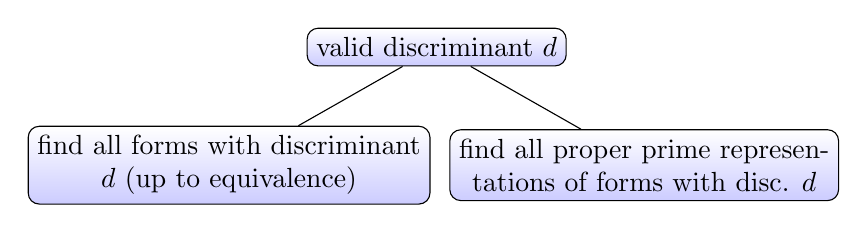
\begin{tikzpicture}[sibling distance=15em,
  every node/.style = {shape=rectangle, rounded corners,
    draw, align=center,
    top color=white, bottom color=blue!20}]]
  \node {valid discriminant $d$}
    child { node {find all forms with discriminant\\ $d$  (up to equivalence)}}
    child { node {find all proper prime represen-\\tations of forms with disc. $d$}};
    \end{tikzpicture}
\end{equation*}
(Recall we use Theorem 4 mostly in the form of Corollary 5.) As we need Theorem 7 for the tasks above, a \textbf{valid} discriminant is one that is nonsquare with $d \equiv 0, 1$ (mod $4$). The last condition guarantees the existence of forms with discriminant $d$ (by Theorem 4).

\subsubsection{}
Rule of Thumb: If there are 1 or 2 forms with discriminant $d$ (up to \textbf{proper} equivalence), one can hope to find the proper prime representations of each form with further analysis. This is illustrated in the next subsection.
\begin{remark}
    Here is one of the strange places where proper equivalence behaves better than just equivalence. The reason is a little out of scope.
\end{remark}

\subsection{Example}
Consider the forms with $d = -20$. Applying (9), we find that the only reduced forms with discriminant $d = -20$ are
\begin{equation*}
    x^{2} + 5y^{2}, \quad 2x^{2}+2xy+3y^{2}, \quad 2x^{2}-2xy+3y^{2}.
\end{equation*}
It is not hard to see the last two are properly equivalent, so all forms with discriminant $d$ are (properly) equivalent to
\begin{equation}
    x^{2} + 5y^{2}, \quad 2x^{2}+2xy+3y^{2}.
\end{equation}
By Corollary 5, the primes properly represented by equations in (11) are those that are
\begin{equation*}
    p \equiv 1, 3, 7, 9 \pmod{20}.
\end{equation*}
The first equation can only represent numbers $0, 1, 4$ (mod $5$) and the second equation can only represent numbers $0, 2, 3$ (mod $5$). Further analysis gives:
\begin{itemize}
    \item $x^{2} + 5y^{2}$ properly represents all primes 1, 9 (mod $20$)
    \item $2x^{2}+2xy+3y^{2}$ properly represents all primes 3, 7 (mod $20$)
\end{itemize}
\end{document}